\documentclass[a4paper, 11pt, titlepage]{article}
\usepackage{fancyhdr}
\usepackage{graphicx}
\usepackage{imakeidx}
\usepackage{makeidx}
\usepackage{mathtools}
\usepackage[spanish]{babel}
\usepackage{eurosym}
\usepackage{hyperref}
\usepackage{amssymb}
\usepackage{listings}
\usepackage{xcolor}
\usepackage{mathtools}
\usepackage{blkarray, bigstrut}
\usepackage{stackrel} 

\title{Estructura de computadores}
\author{Francisco Javier Balón Aguilar}

\begin{document}

\maketitle
\renewcommand{\contentsname}{Índice}
\tableofcontents
\newpage

\section{Unidad Central de Proceso (CPU)}\label{cpu}

    \subsection{Máquina de Von Neumann}

        La máquina de Von Neumann (1945) es un modelo computacional teórico referencia para 
        el diseño de arquitecturas de ordenadores.

        El modelo propone una unidad central de proceso (véase sección \ref{cpu}), que controla y gobierna la lógica 
        de la máquina, una memoria (véase sección \ref{memoria}) que contendrá instrucciones y datos, una unidad de entrada
        y salida (véase sección \ref{entradasalida}) que gestionará las entradas y salida de resultados, y un conjunto de periféricos.

        \begin{figure}[htp]
            \centering
            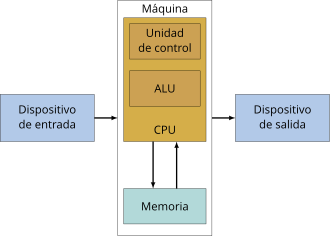
\includegraphics[width=0.7\textwidth]{resources/vonneumann.png}
            \caption{Diagrama del modelo de arquitectura von Neumann.}
            \label{vonneumann}
        \end{figure}

    \subsection{Ciclo Básico de Instrucciones}

        \subsubsection{Registros y operaciones básicas}

        \subsubsection{Instrucciones, operaciones y órdenes}

        \subsubsection{Tipo de instrucciones}

    \subsection{La Unidad de Control}

    \subsection{Unidad Aritmético-Lógica}

    \subsection{Modos de direccionamiento}

\section{Memoria}\label{memoria}
\section{Módulo de Entrada y Salida}\label{entradasalida}
\section{Buses}

\end{document}